\documentclass[3p]{elsarticle}
\usepackage{ae,aecompl}
\usepackage[T1]{fontenc}
\usepackage[utf8]{inputenc}
\usepackage{pgfplots}
\usepackage{pst-plot}
\usepackage{tikz}
\usepgfplotslibrary{external}
\tikzexternalize
\usepackage{amsmath}
\usepackage{amssymb}
\usepackage{gensymb}
\usepackage{upgreek}
\usepackage{float}
\usepackage{indentfirst}
\parskip=0pt

\begin{document}

\begin{frontmatter}

\title{Spatio-temporal Scanning Electrochemical Microscopy}
\cortext[cor]{Corresponding author}
\author[akiss]{András Kiss\corref{cor}}
\address[akiss, gnagy]{Department of General and Physical Chemistry, Faculty of Sciences, University of Pécs, 7624 Pécs, Ifjúság útja 6, Hungary}
%\address[akiss, gnagy]{János Szentágothai Research Centre, University of Pécs, 7624 Pécs, Ifjúság Útja 20, Hungary}
\ead{akiss@gamma.ttk.pte.hu}
\author[dfilotas]{Dániel Filotás}
\ead{filotasdaniel@gmail.com}
\author[gnagy]{Géza Nagy}
\ead{g-nagy@gamma.ttk.pte.hu}


\begin{abstract}

Scanning Electrochemical Microscopy (SECM) and SIET above all else, is a technique to be used to gather information in the spatial domain about a particular system of interest.
Even when a time coordinate is assigned to a spatial scan, it is always assigned to the scan as a whole, without any temporal distinction between the individual data points.
These however, could have very different time coordinates, because SECM is relatively slow.
Scan times are often measured in minutes, during which a dynamic system changes dramatically.
The difference between the actual, and the assigned time coordinate could lead to difficulties during evaluation.
 
This paper proposes mixed domain scanning.
During the scan, the time coordinates of each individual data acquisition points are stored as well as the spatial ones.
From the data, interesting new, spatiotemporal plots can be assembled, which can be used to study dynamically changing systems, and answer questions like how a species of ion is distributed in the system, and how does that distribution change in time.
As an example, consecutive scans were recorded on a pre-defined line above a galvanically corroding magnesium sample, and the distribution of hydrogen ions were monitored in time along that line.

Ide még azt kéne leírni, hogy nagy térbeli ÉS időbeli felbontás az SECM-mel lehetetlen, mert a nagy térbeli felbontáshoz sok pont kell, ami sok időbe telik.
Mivel sok időbe telik, csak alacsony frekvenciával készíthetőek teljes képek.
Ezért néha csak egyes vonalpásztázásokat alkalmaznak, hogy növeljék az időbeli felbontást - pl. korai korróziós események nyomon követésére - és az EGÉSZ vonalhoz egy időpillanatot rendelnek hozzá.
Még ez is torzított képet ad a rendszerről, hiszen a vonal pontjai nem egy időben lettek felvéve.
Egy másik megközelítés egy érdekes pont kitüntetése, és a jel követése ezen a ponton, ilyenkor természetesen abszolút nincs térbeli felbontás.


\end{abstract}
\begin{keyword}
	scanning electrochemical microscopy \sep potentiometry \sep spatiotemporal \sep mixed domain scanning
\end{keyword}
\end{frontmatter}

\section{Introduction}
Citation \cite{artefacts}.


\begin{figure}
\centering
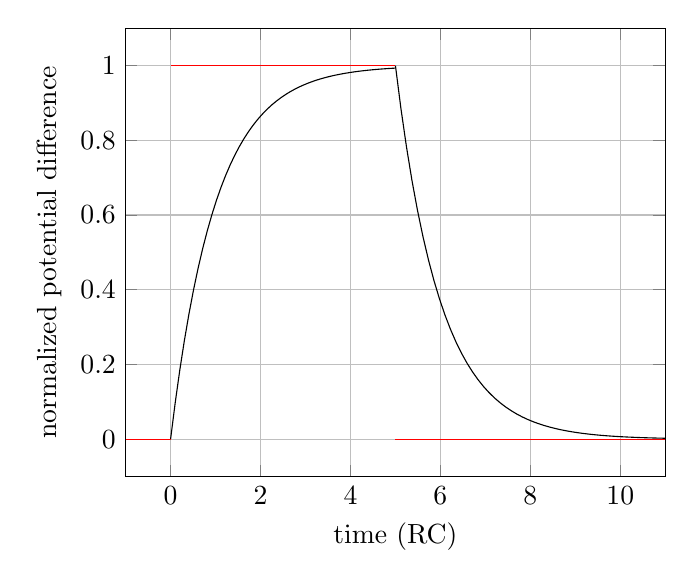
\begin{tikzpicture}
\begin{axis}[xmin=-1,xmax=11,ymin=-0.1,ymax=1.1,xlabel={time (RC)}, ylabel={normalized potential difference},no markers,samples=50,grid=both]
        \addplot[domain=0:5, black] {1-exp(-x)};
        \addplot[domain=-1:0, red] {0};
        \draw [color=red, dashed] (10,10) -- (10,110);
        \addplot[domain=0:5, red] {1};
        \addplot[domain=5:11, black] {exp(-x+5)};
        \draw [color=red, dashed] (60,10) -- (60,110);
        \addplot[domain=5:11, red] {0};
        \draw [color=red, fill=white] (10,10) circle [radius=0.1cm];
        \draw [color=red, fill=white] (10,110) circle [radius=0.1cm];
        \draw [color=red, fill=red] (10,60) circle [radius=0.1cm];
        \draw [color=red, fill=white] (60,10) circle [radius=0.1cm];
        \draw [color=red, fill=white] (60,110) circle [radius=0.1cm];
        \draw [color=red, fill=red] (60,60) circle [radius=0.1cm];
        \draw [color=black, fill=black] (20,73.2) circle [radius=0.1cm] node[right] {0.632};
        \draw [color=black, fill=black] (40,105) circle [radius=0.1cm] node[below] {0.95};
        \draw [color=black, fill=black] (70,46.8) circle [radius=0.1cm] node[right] {0.368};
        \draw [color=black, fill=black] (90,15) circle [radius=0.1cm] node[above] {0.05};
\end{axis}
\end{tikzpicture}
\caption[Charging and discharging the series $RC$ circuit.]{Charging and discharging the series $RC$ circuit.
Red: normalized input voltage ($V_{in}$) to the series $RC$ circuit, two consecutive \emph{Heaviside step functions}, the second one is inversed and shifted $5RC$ to the right.
Black: normalized output voltage ($V_{out}$) of the series $RC$ circuit.}
\label{fig:charge_discharge}
\end{figure}


\section{Theory}
Eq. \ref{eq:rc} describes the transient cell response when the measuring electrode is brought to contact with a solution of different analyte activity.

\begin{equation}
\label{eq:rc}
	E_{cell}(t) = E_{cell}(\infty) + [E_{cell}(0) - E_{cell}(\infty)]e^{-t/RC}
\end{equation}

\section{Material and methods}
\section{Results and discussion}

%%%%%%%%%%%%%%%%%%%%%%%%%%%%%%% FIGURE EXAMPLE %%%%%%%%%%%%%%%%%%%%%%%%%%%%%%%%%%
\def\s{0.25}
\begin{figure}
\centering
% trim = top left bottom right
\includegraphics[trim = 10mm 20mm 0mm 10mm, clip, width=\s\textwidth, angle=-90]{gnuplot_2d.eps}\includegraphics[trim = 10mm 20mm 0mm 10mm, clip, width=\s\textwidth, angle=-90]{gnuplot_2d.eps}\includegraphics[trim = 10mm 20mm 0mm 10mm, clip, width=\s\textwidth, angle=-90]{gnuplot_2d_deconvoluted.eps}
\caption{Caption.}
\label{fig:label1}
\end{figure}

\begin{figure}
\centering
% trim = top left bottom right
\includegraphics[width=\s\textwidth, angle=-90]{test.eps}

\includegraphics[width=\s\textwidth, angle=-90]{test_deconvoluted.eps}
\caption{Caption.}
\label{fig:label1}
\end{figure}


%%%%%%%%%%%%%%%%%%%%%%%%%%%%%%% TABLE EXAMPLE %%%%%%%%%%%%%%%%%%%%%%%%%%%%%%%%%%
\begin{table}
                \caption{Comparison of the scanning algorithms.}
                \label{table:comp}
                \centering
                \begin{tabular}{r c c c}
                        Algorithm & Number of sampling points & Total scan time (s) & Mean squared error \\
                        \hline
                        Meander & 441 & 440 & $2.75\times 10^{-2}$ \\
                        Fast comb & 441 & 520  & $2.07\times 10^{-2}$ \\
                        Comb & 441 & 881 & $2.75\times 10^{-2}$ \\
                        Web & 110 & 109 & $9.63\times 10^{-3}$ \\
                        Arc & 341 & 340 & $2.95\times 10^{-3}$ \\

                \end{tabular}

\end{table}

\section{Conclusions}
\section*{Acknowledgements}
This research was supported by the European Union and the State of Hungary, co-financed by the European Social Fund in the framework of T\'{A}MOP-4.2.4.A/ 2-11/1-2012-0001 'National Excellence Program' and T\'{A}MOP-4.2.2.A-11/1/KONV-2012-0065.

\section*{References}

\begin{thebibliography}{5}

\bibitem{artefacts}P. J. Eaton, P. West. Atomic force microscopy. Vol. 10. Oxford: Oxford University Press, 2010.

\end{thebibliography}

\end{document}
